\chapter{Introduction and geometry}

What are elliptic curves and why are they important? See Andrew Sutherland's slides~\url{http://math.mit.edu/classes/18.783/Lecture1.pdf} for an introduction.

In this chapter we'll present an elementary, computational approach side by side with a more theoretical, geometric approach. (The reader may choose to focus on one or the other.)

\section{Definition and motivations}

An elliptic curve is essentially the ``next simplest curve" besides a conic. We give two definitions of an elliptic curve which make this precise.
\begin{df}[Elementary definition]\llabel{df:ec1}
%\begin{enumerate}
%\item
An \textbf{elliptic cuve} $E$ over a field $K$ is the projective closure of a plane affine curve \[y^2=f(x)\] with a specified rational point (typically the point at infinity). 
Here, $f\in K[x]$ is a monic cubic polynomial with distinct roots in $\ol K$.\footnote{When $\chr(K)=2$, we have to allow equations of the form $y^2+a_1xy+a_3y=f(x)$. More on this when we talk about the Weierstrass form.}
%\item For any field extension $L/K$, let
%\[
%E(L)=\set{(x,y)\in L}{y^2=f(x)}\cup\{O\}.
%\]
%\end{enumerate}
\end{df}

\begin{df}[Algebraic geometry definition]\llabel{df:ec2}
An \textbf{elliptic curve} $E$ over a field $K$ is a smooth projective curve of genus 1 with a distinguished point in $K$.
\end{df}

Why is this interesting to study? We give an example of a problem where elliptic curves naturally arise.

%\subsection{Problems involving elliptic curves}

\subsection{The congruent number problem}
As elliptic curves are the ``next simplest curves" apart from conics, and there is a lot more freedom for elliptic curves, it is natural that a lot of Diophantine equations reduce to problems about elliptic curves. This is a large part of the motivation for studying them.

One famous still unsolved Diophantine equation is the congruent number problem, which we'll now consider. See Keith Conrad's article at \url{http://www.thehcmr.org/issue2_2/congruent_number.pdf} for an in-depth discussion, and~\cite{Ko84} for the approach to the problem using modular forms.

%\section{Fermat's method of descent}
Consider a right triangle $\triangle$ with legs $a$, $b$, and hypotenuse $c$. It satisfies the following.
\begin{align*}
a^2+b^2&=c^2\\
\Area(\triangle)&=\rc2ab.
\end{align*}
\begin{df}
We say
\begin{enumerate}
\item
$\triangle$ is \textbf{rational} if $a,b,c\in \Q$. 
\item
$\triangle$ is \textbf{primitive} if $a,b,c\in \Z$ and $\gcd(a,b,c)=1$. (This is the same as saying that $a,b,c$ are pairwise coprime.)
\end{enumerate}
\end{df}
Recall the following parametrization.
\begin{lem}[Rephrasing Theorem~\ref{thm:pythag}]\llabel{lem:primitive-triangle}
Every primitive triangle is of the form $(u^2-v^2,2uv,u^2+v^2)$ for $u,v\in \Z$ where $u>v>0$.
\end{lem}
\begin{df}
$D\in \Q^+$ is \textbf{congruent} if it is the area of some rational right-angled triangle.
%equivalent to AS of three terms.
\end{df}
Note that it suffices to consider squarefree integers $D\in \N$ since they form a coset of $\Q^{\times 2}$ in $\Q$.

For example, 5 and 6 are congruent.

\thbox{\begin{lem}\llabel{lem:cong-iff-ell}
$D\in \Q^+$ is congruent iff $Dy^2=x^3-x$ for some $x,y\in \Q$ with $y\ne 0$, iff $y^2=x^3-D^2x$ for some $y\ne 0$.
\end{lem}}

Thus the problem of whether or not a number is congruent is equivalent to whether or not there exists a 

\begin{proof}
We first show the first two conditions are equivalent. 
Suppose $D$ is congruent. 
Then there is $w$ such that $Dw^2$ is the area of a primitive triangle. 
By lemma~\ref{lem:primitive-triangle}, we can write the sides in the form $u^2-v^2$, $2uv$, and $u^2+v^2$ for $u,v,w\in \Q$. Then
\begin{align*}
Dw^2&=\rc2(u^2-v^2)2uv\\
D\pf{w}{v^2}^2&=\pf uv\pa{\pf uv^2-1}.
\end{align*}
Set $x=\fc uv$ and $y=\fc{w}{v^2}$. Conversely, given $x,y$, let $u,v$ be the numerator and denominator of $x$, and let $w=yv^2$.

To go between $Dy^2=x^3-x$ and $y^2=x^3-D^2x$, make the substitution $y\mapsfrom \fc{y}{D^2}$ and $x\mapsfrom \fc{x}{D}$.
\end{proof}
Fermat showed $D=1$ is not congruent.
\begin{thm}\llabel{thm:1-not-cong}
There are no solutions to
\begin{equation}\llabel{eq:no-soln-1-cong}
w^2=uv(u-v)(u+v)
\end{equation}
for $u,v,w\in \Z$. Hence 1 is not a congruent number.
\end{thm}
\begin{proof}
An elementary approach is to use infinite descent. See the notes at~\url{https://dl.dropboxusercontent.com/u/27883775/math\%20notes/part_iii_elliptic.pdf}.
%Without loss of generality $w>0$. We can replace $(u,v)$ by $(-u,-v)$, $(-v,u)$, or $(v,-u)$, so  we can assume $u,v>0$. WLOG $\gcd(u,v)=1$; then $\gcd(u,u\pm v)=1$ as well. If a prime $p\mid u-v$ and $p\mid u+v$ then $p\mid 2u$ and $p\mid 2v$. Thus the only possible common factor among $u,v,u+v,u-v$ is 2, and this happens when $u\equiv v\pmod 2$.
%
%If $u\equiv v\pmod 2$, replace $(u,v,w)$ with $\pa{\pf{u+v}{2},\pf{u-v}{2},\fc{w}{2}}$. Now our new $u,v$ are coprime, or else $u,v$ are divisible by 2, in which case we divide it out.
%
%Thus we can assume $u\nequiv v\pmod 2$, so $u,v,u\pm v$ are coprime integers.
%
%By unique factorization of $\Z$,
%\begin{align*}
%u&=a^2\\
%v&=b^2\\
%u+v&=c^2\\
%u-v&=d^2
%\end{align*}
%for some $a,b,c,d\in \Z$. Since $u\nequiv v\pmod 2$, $c\equiv d\equiv 1\pmod 2$. Now
%\[
%\pf{c+d}{2}^2+\pf{c-d}{2}^2=\fc{c^2+d^2}2=a^2
%\]
%so $\pa{\fc{c+d}2,\fc{c-d}2,a}$ is a primitive triangle. %check
%The area is $\rc2\cdot \fc{c^2-d^2}4=\fc{2v}{8}=\fc{v}{4}=\pf b2^2$.
%
%Let $w_1=\fc b2$. By Lemma~\ref{lem:primitive-triangle} again, $w_1^2=u_1v_1(u_1^2-v_1^2)$ for some $u_1,v_1\in \Z$. This is another solution to~\eqref{eq:no-soln-1-cong}. We have $4w_1^2=b^2=v$. By the original equation, $v\mid w^2$ so $v\le w^2$, giving
%\[
%4w_1^2\le w^2\implies w_1\le \fc{w}{2}<w.
%\]
%We are done by Fermat's method of infinite descent.
\end{proof}

\section{The equation of an elliptic curve}
\subsection{Every elliptic curve can be put in Weierstrass form}
We would like to have some ``standard form" for an elliptic curve, that is
\begin{enumerate}
\item
a form involving as few terms as possible, such that every elliptic curve is isomorphic to an elliptic curve in that form, and
\item
an easy way to tell if two elliptic curves in that form are isomorphic.
\end{enumerate}
We'll investigate two natural forms for an elliptic curve: the Weierstrass and Legendre forms.
\begin{df}
A \textbf{(long) Weierstrass equation} is an eqution in the following form
\begin{align*}
\text{affine coordinates}&& y^2+a_1xy+a_3y&=x^3+a_2x^2+a_4x+a_6\\
\text{projective coordinates}&& Y^2Z+a_1XYZ+a_3YZ^2&=X^3+a_2X^2Z+a_4XZ^2+a_6Z^3
\end{align*}
A \textbf{(short) Weierstrass equation} is an equation in the following form
\begin{align*}
\text{affine coordinates}&& y^2=x^3+Ax+B\\
\text{projective coordinates}&& Y^2Z=X^3+AXZ^2+BZ^3.
\end{align*}
\end{df}
A note on the numbering in the coefficients: they are the weights for the coefficients that make the equation $y^2+a_1xy+a_3y=x^3+a_2x^2+a_4x+a_6$ homogeneous if $y$ has weight 3 and $x$ has weight 2.

Our main theorem in this section is the following. (The proof may be safely skipped for an elementary course, by using Definition~\ref{df:ec1} for an elliptic curve.)
\begin{thm}\llabel{thm:cam3-1}
Every elliptic curve $E$ is isomorphic over $K$ to a curve in Weierstrass form, via an isomorphism mapping $O_E\mapsto (0:1:0)$.
\end{thm}
%Our previous lemma~\ref{lem:cam2-7} was a special case: $E$ was a smooth plane cubic and $O_E$ a point of inflection. This is more general because it's an arbitrary curve of genus 1, and the point may not be a point of inflection.
\begin{fct}
Let $D$ be a divisor on $E$, i.e., a formal sum of $\ol K$-points on $E$. If $D$ is defined over $K$ (i.e., $D$ is fixed by the action of $G(\ol K/K)$), then $\cL(D)$ has a basis consisting of rational functions defined over $K$, not just in $\ol K(E)$. \fixme{Proof?}
\end{fct}
\begin{proof}[Proof of Theorem~\ref{thm:cam3-1}]
\ul{Step 1:}
The idea is that if we pick some functions $x,y$ to be our coordinates, by Riemann-Roch, we will get a linear dependence relations between terms $x^iy^j$ before too long.
\begin{enumerate}
\item
$\cL(2O_E)$ is 2-dimensional by Riemann-Roch~\ref{thm:rr-ec}. Pick a basis $1,x$.
\item $\cL(3O_E)$ is 3-dimensional by Riemann-Roch. Extend to a basis $1,x,y$.
\item
Look at the elements $1,x,y,x^2,xy,x^3,y^2$: these are all in $\cL(6,O_E)$. But the dimension of the space is 6 and there are 7 elements, so there is a linear dependence relation.

Leaving out either $x^3$ or $y^2$ gives a basis for $\cL(6O_E)$ since each term has a different order pole at $O_E$. Thus the coefficients of $x^3$ and $y^2$ are nonzero. Rescaling $x$ and $y$ we get
\[
y^2+a_1xy+a_3y=x^3+a_2x^2+a_4x+a_6
\] 
for some $a_i\in K$.
%(If $E$ is defined over $K$, then $a_i\in K$.)
\end{enumerate}
We obtain a rational map
\begin{align*}
\phi:E&\to E'\subeq \Pj^2\\
P&\mapsto [x(P):y(P):1].
\end{align*}
A rational map from a smooth curve to a smooth curve is always a morphism (Theorem~\ref{thm:rat-morphism}).

\ul{Step 2:} We show $\phi$ is an isomorphism by showing its degree is 1. By Theorem~\ref{thm:cam2-8} \fixme{(how?)} on the point $\iy\in \Pj^1$ with inverse $O_E$ under $x,y$, we have

\begin{align*}
[K(E):K(x)]&=\deg(E\xra{x}\Pj^1)=\ord_{O_E}\prc x=2\\
[K(E):K(y)]&=\deg(E\xra{y}\Pj^1)=\ord_{O_E}\prc y=3.
\end{align*}
We write down the fields involved.
\[
\xymatrix{
& K(E)\ls{rdd}^3\ls{d} &\\
& K(x,y) \ls{rd} &\\
K(x)\ls{uur}^2\ls{ur} && K(y)
}
\]
The tower law says that $[K(E):K(x,y)]$ divides 2 and 3 so $K(E)=K(x,y)$ thus $\phi^*K(E')=K(E)$ and $\deg (\phi)=1$. Thus $\phi$ is birational.

We know $E$ is projective, and we need $E'$ to be smooth. If $E'$ is singular, we can find a rational parametrization, so $E$ and $E'$ are rational. This is a contradiction because $E$ has genus 1.

Thus $E'$ is smooth and $\phi$ is an isomorphism.

We check the image of $O_E$. Since $x$ has a pole of order 2 at $O_E$ and $y$ has a pole of order 3,
\begin{align*}
\phi:E&\to E'\\
P&\mapsto \ba{\fc xy(P):1:\rc y(P)}\\
O_E&\mapsto [0:1:0].
\end{align*}
\end{proof}

\subsection{Transforming an elliptic curve}
We can use the proof of Theorem~\ref{thm:cam3-1} to find when 2 curves in Weierstrass form are isomorphic.
\begin{pr}\llabel{pr:cam3-2}
Let $K$ be algebraically closed.
Let $E,E'$ be elliptic curves over $K$ in Weierstrass form. Then $E\cong E'$ over $K$ iff the equations are related by substitutions 
\begin{align*}
x&=u^2x'+r\\
y&=u^3y'+u^2sx'+t
\end{align*}
for some $r,s,t,u\in K$ with $u\ne 0$.
\end{pr}
%specified pt on E to E'
\begin{proof}
Because $x,y$ and $x',y'$ are Weierstrass coordinates, we must have $x,x'\in \cL(2O_E)$ and $y,y'\in \cL(3O_E)\bs \cL(2O_E)$. %Look at the previous proof: how much freedom did we have when picking $x$ and $y$? 

Again by Riemann-Roch, we have
\[
\an{1,x}=\cL(2O_E)=\an{1,x'}.
\]
From this we see $x=\la x'+r$ for some $\la,r\in K$. Similarly,
\[
\an{1,x,y}=\cL(3O_E)=\an{1,x',y'}
\]
and hence $y=\mu y' +\si x' + t$ for some $\mu,\si,t\in K$ and $\mu\ne 0$. Looking at coefficients of $y^2$ and $x^3$ we need $\la^3=\mu^2$, so $\la=u^2$ and $\mu=u^3$ for some $u\in K$. Put $s=\fc{\si}{u^2}$.
\end{proof}
\fixme{A warning when $K$ is not algebraically closed: we can have curves isomorphic over $\ol K$ but not $K$. Quadratic, cubic, sextic twists.}

A Weierstrass equation defines an elliptic curve iff it defines a smooth curve, iff $\De(a_1,\ldots, a_6)\ne 0$ where $\De\in \Z[a_1,\ldots, a_6]$ is a certain polynomial (see the formula sheet!).

If $\chr(K)\ne 2,3$, we can reduce to the case $y^2=x^3+ax+b$, with discriminant
\[
\De=-16(4a^3+27b^2).
\]
(this is 16 times the usual formula for the discriminant of a polynomial).

\begin{cor}\llabel{cor:cam3-3}
Assume $\chr(K)\ne 2,3$. The elliptic curve 
\begin{align*}
E:y^2&=x^3+ax+b\\
E':y^2&=x^3+a'x+b'
\end{align*}
\end{cor}
are isomorphic over $K$ iff $a'=u^4a$ and $b'=u^6b$ for some $u\in K^*$.
\begin{proof}
$E$ and $E'$ are related by a substition as in Proposition~\ref{pr:cam3-2} with $r=s=t=0$. 
\end{proof}

%\subsubsection{Change of coordinates}


\subsection{Legendre form}
Another useful for an elliptic curve is the \textbf{Legendre form}.
\begin{lem}\llabel{lem:cam2-7}
Let $C\sub \Pj^2$ be a smooth plane cubic, and $P\in C$ a point of inflection. Then we can change coordinates such that
\[
C:Y^2Z=X(X-Z)(X-\la Z),\qquad \la\ne 0,1,\qquad P=(0:1:0).
\]
\end{lem}
\begin{proof}
We change coordinates %use a 3x3 invertible matrix
such that $P=(0:1:0)$ and $T_pC=\{Z=0\}$. Then
\[
C:\{F(X,Y,Z)=0\}\sub \Pj^2.
\]
A point of inflection means the line meets the curve with multiplicity 3, so we get a triple root
\[
F(t,1,0)=ct^3.
\]
Thus there are no terms $X^2Y,XY^2, Y^3$. Thus
\[
F\in \an{Y^2Z,XYZ,YZ^2,X^3,X^2Z,XZ^2, Z^3},
\]
with the coefficient of $Y^2Z$ nonzero (otherwise $P\in C$ would be singular \fixme{why?}), otherwise everything is divisible by $Z$, and $C$ contains $\{Z=0\}$ (curves are irreducible).
%why is reducibility preserved

We can rescale $X,Y,Z,F$, so WLOG
\[
C:Y^2Z+a_1XYZ+a_3YZ^2=X^3+a_2X^2Z+a_4XZ^2+a_6Z^3.\qquad \text{Weierstrass form}
\]
Substituting $Y\lar Y-\rc2 a_1X-\rc 2 a_3Z$ (completing the square) we may assume $a_1=a_3=0$ (we assume $\chr(K)\ne 2$), giving
\[
C: Y^2Z=Z^3f\pf{X}{Z}.
\]
$C$ is smooth, so $f$ has distinct roots, without loss of generality, 0, 1, $\la$. Thus
\[
C: Y^2Z=X(X-Z)(Z-\la Z).\qquad \text{Legendre form}
\]
\end{proof}



\subsection{Invariants of an elliptic curve}

\fixme{Motivate the $j$-invariant. Quotient of 2 things with weight 12.}

\begin{df}\llabel{df:j-inv}
The \textbf{$j$-invariant} of $E$ is
\[
j(E)=\fc{1728(4a^3)}{4a^3+27b^3}.
\]
\fixme{Also define the discriminant and invariant differential.}
\end{df}
\begin{cor}
$E\cong E'$ implies $j(E)=j(E')$ and the converse holds over $K=\ol K$. 
\end{cor}
\begin{proof}
We have $E\cong E'$ iff $a'=u^4a$, $b'=u^6b$ for some $u\in K^*$. This implies $(a^3:b^2)=((a')^3:(b')^2)$, which is true iff $j(E)=j(E')$. The converse holds if the field is algebraically closed (we need to extract roots).
\end{proof}


\subsection{Singular cubics}
[Weierstrass form, etc.]



\section{Group law}
There is a natural group law on elliptic curve. There are several ways to think about it.
\begin{enumerate}
\item
The key point here is that every line intersects an elliptic curve in 3 points, counted with multiplicity.
Given two points $P$ and $Q$ on an elliptic curve $E$, let the third point of intersection be $-(P+Q)$ (and its reflection across the $x$-axis be $P+Q$). We can obtain explicit expressions for $P+Q$.
\item 
Every algebraic curve has a group associated with it, the group of divisors. It turns out that the divisor class group of an elliptic curve can be put in direct correspondence to the points on the elliptic curve.
\item
For an elliptic curve over $\C$, we can define the group law by finding some analytic map $\C\to E(\C)$. Then addition on $\C$ pushed forward gives a group law on $E$. This is just like the fact that the addition formulas for $\sin,\cos$ give a group law on the circle. We'll see this in the chapter on elliptic curves over $\C$.
\end{enumerate}

\subsection{Elementary approach, I}

The following is an adaptation of the proof in \cite[p.\ 28]{Cassels}. The proof is nice, but fails to capture all cases, so we will give a more correct, but messier, proof later.

\begin{thm*}
Let $P$, $Q$, and $R$ be three points on an elliptic curve $E(K)$ for some field $K$ that we may assume is algebraically closed.
Assume that $P$, $Q$, $R$, and the zero point $O$ are all in \emph{general position} (this means that in the diagram below there are no relationships among the points other than those that necessarily exist by construction). Then
\[
(P+Q)+R=P+(Q+R).
\]
\end{thm*}
\begin{proof}
The line $\ell_0$ through $P$ and $Q$ meets the curve $E$ at a third point, $-(P+Q)$, and the line $m_2$ through $O$ and $-(P+Q)$ meets $E$ at $P+Q$.
Similarly, the line $m_0$ through $P$ and $R$ meets $E$ at $-(P+R)$, and the line $\ell_2$ through $O$ and $-(P+R)$ meets $E$ at $P+R$.
Let $S$ be the third point where the line $\ell_1$ through $Q+P$ and $R$ meets $E$, and let $T$ be the third point where the line $m_1$ through $Q$ and $P+R$ meets $E$.  See the diagram below.

\begin{center}
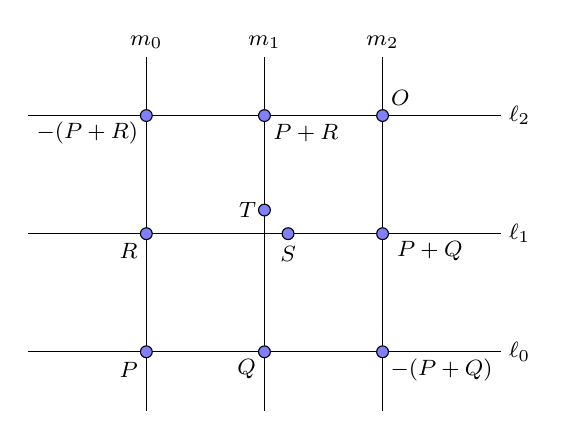
\begin{tikzpicture}[scale=1.5]
\footnotesize
\foreach \x in {0,1,2} \draw[black] (\x,-0.5) -- (\x,2.5) node[above] {{$m_\x$}};
\foreach \y in {0,1,2} \draw[black] (-1,\y) -- (3,\y) node[right] {{$\ell_\y$}};
\foreach \x in {0,1,2} \foreach \y in {0,2} \draw[fill=blue!50] (\x,\y) circle (0.05);
\foreach \x in {0,2} \draw[fill=blue!50] (\x,1) circle (0.05);
\draw[fill=blue!50] (1.2,1) circle (0.05) node at (1.2,0.83) {{$S$}};
\draw[fill=blue!50] (1,1.2) circle (0.05) node[left] {{$T$}};
\node at (-0.15,-0.15) {{$P$}};
\node at (0.85,-0.15) {{$Q$}};
\node at (2.5,-0.15) {{$-(P+Q)$}};
\node at (-0.15,0.85) {{$R$}};
\node at (2.4,0.85) {{$P+Q$}};
\node at (-0.5,1.85) {{$-(P+R)$}};
\node at (1.35,1.85) {{$P+R$}};
\node at (2.15,2.15) {{$O$}};
\end{tikzpicture}
\end{center}

We have $S=-(Q+P)+R$ and $T=-(Q+(P+R))$.  It suffices to show $S=T$.
Suppose~not.
Let $g(x,y,z)$ be the cubic polynomial formed by the product of the lines $\ell_0,\ell_1,\ell_2$ in homogeneous coordinates,
and similarly let $h(x,y,z)=m_0m_1m_2$.
We may assume $g(T)\ne 0$ and $h(S)\ne 0$, since the points are in general position and $S\ne T$.
Thus $g$ and $h$ are linearly independent elements of the $k$-vector space $V$ of homogeneous cubic polynomials in $k[x,y,z]$.
The space $V$ has dimension 10, thus the subspace of homogeneous cubic polynomials that vanish at the eight points $O$, $P$, $Q$, $R$,
$\pm(Q+P)$, and $\pm(P+R)$ has dimension 2 and is spanned by $g$ and $h$.
The homogeneous polynomial $f(x,y,z)=x^3+Axz^2+Bz^3-zy^2$ that defines $E$ is a nonzero element of this subspace, so we may write $f=ag+bh$ as a linear combination of $g$ and $h$.
But $f(S)=f(T)=0$, since $S$ and $T$ are both points on $E$, which implies that $a$ and $b$ are both zero.
This contradicts the linear independence of $g$ and $h$, since $f$ is not the zero polynomial.
\end{proof}
\subsection{Elementary approach, II: The group law in algebraic terms}
Let $P=(x_1,y_1,z_1)$ and $Q=(x_2,y_2,z_2)$ be two points on $E$.
We will compute the sum $P+Q=R=(x_3,y_3,z_3)$ by expressing the coordinates of $R$ as rational functions of the coordinates of $P$ and $Q$.
If either $P$ or $Q$ is the point at infinity, then $R$ is simply the other point, so we assume that $P$ and $Q$ are affine points with $z_1=z_2=1$.
There are two cases:
\begin{description}
\item[Case 1.] $x_1\neq x_2$. The line $\overline{PQ}$ has slope
  $m=(y_2-y_1)/(x_2-x_1)$, which yields the equation $y-y_1=m(x-x_1)$.
  The point $-R=(x_3,-y_3,1)$ is on this line, thus $-y_3=m(x_3-x_1)+y_1$.
  Substituting for $y_3$ in the Weierstrass equation for $E$ yields
  $$(m(x_3-x_1)+y_1)^2=x_3^3+Ax_3+B.$$
  Simplifying, we obtain $0=x_3^3-m^2x_3^2+\cdots$, where the ellipsis hides lower order terms.
  The values $x_1$ and $x_2$ satisfy the same cubic equation, and the quadratic coefficient $-m^2$
  must be the sum of the roots.  Thus $x_3=m^2-x_1-x_2$.  To sum up, we have
\begin{align*}
m &= \fc{y_2-y_1}{x_2-x_1},\\
x_3 &= m^2-x_1-x_2,\\
y_3&=m(x_1-x_3)-y_1.
\end{align*}
  Thus to compute $P+Q=R$, we need one inversion and three multiplications (one of which is a squaring).
  We'll denote this cost 3M+I.

\item[Case 2.] $x_1=x_2$. If $y_1\neq y_2$, then they must be opposite
  points and $R=0$. Otherwise $P=Q$, and we compute the slope of the
  tangent line by implicitly differentiating the Weierstrass equation for $E$.
  This yields $2y\dy=3x^2\dx+A\dx$, so 
\[m=\frac{dy}{dx}=\frac{3x_1^2+A}{2y_1}.\]
  The formulas for $x_3$ and $y_3$ are then the same as
  the previous case.  Note that we require an extra multiplication here,
  so computing $R=2P$ has a cost of 4M+I.
\end{description}

With these equations in hand, we can now prove associativity as a formal
identity, treating $x_1,y_1,z_1,x_2,y_2,z_2,x_3,y_3,z_3,A,B$ as indeterminants
subject to the three relations implied by the fact that $P$, $Q$, and
$R$ all lie on the curve $E$.  See the Sage worksheet
\begin{center}
\url{https://hensel.mit.edu:8002/home/pub/1/}
\end{center}
for details, which includes checking all the special cases.

The equations above can be converted to projective coordinates by replacing $x_1,y_1,x_2$, and $y_2$ with
$x_1/z_1$, $y_1/z_1$, $x_2/z_2$, and $y_2/z_2$ respectively, and then writing the resulting expressions for $x_3/z_3$ and $y_3/z_3$ with a common denominator.
This has the advantage of avoiding inversions, which are more costly than multiplications (in a finite field of cryptographic size inversions may be 50 or even 100 times more expensive).
This increases the number of multiplications to 12M in case 1
(addition), and 14M in case 2 (doubling).

\subsubsection{Edwards curves*}
There are many alternative representations of elliptic curves that have been proposed.
We give just one example here, Edwards curves \cite{bl,edwards}, which have two significant advantages over Weierstrass equations.
Let $d$ be a non-square element of a field $k$ (assumed to have characteristic not equal to 2, as usual).
Then the equation
\begin{equation*}
x^2+y^2 = 1+dx^2y^2
\end{equation*}
defines an elliptic curve with distinguished point $(0,1)$.\footnote{Technical point: there are two points at infinity, both of which are singular,  violating our requirement that an elliptic curve be smooth.  However, this plane curve can be desingularized by embedding it in $\mathbb{P}^3(k)$.  The points at infinity are then no longer rational, and do not play a role in the group operation on $E(k)$.}
The group operation is given by
\begin{equation*}
(x_3,y_3)=\left(\frac{x_1y_2+y_2x_1}{1+dx_1x_2y_1y_2},\frac{y_1y_2-x_1x_2}{1-dx_1x_2y_1y_2}\right).
\end{equation*}
As written, this involves five multiplications and two inversions (ignoring the multiplication by $d$, which we can choose to be small),
which is greater than the cost of the group operation in Weierstrass form.
However, in projective coordinates we have
\begin{equation*}
\frac{x_3}{z_3}=\frac{z_1z_2(x_1y_2+x_2y_1)}{z_1^2+z_2^2+dx_1x_2y_1y_2},\qquad\frac{y_3}{z_3}=\frac{z_1z_2(y_1y_2-x_1x_2)}{z_1^2+z_2^2+dx_1x_2y_1y_2}\,.
\end{equation*}
There are a bunch of common subexpressions here, and in order to compute $z_3$, we need a common denominator.
Let $r=z_1z_2$, let $s=x_1y_2+x_2y_1$, let $t=dx_1y_2x_2y_1$, and let $u=y_1y_2-x_1x_2$.
We then have
\begin{equation*}
x_3=rs(r^2-t),\qquad y_3=ru(r^2+t),\qquad z_3=(r^2+t)(r^2-t).
\end{equation*}
This yields a cost of 12M, and, if you are clever, you can reduce it to 11M.

The remarkable thing about these formulas is that they handle every case; there
are not separate formulas for addition and doubling, and adding opposite points or the identity element works the same as the general case.
Such formulas are called \emph{complete}, and they have two distinct advantages.
First, they can be implemented very efficiently because there is no branching.
Second, they protect against what is known as a \emph{side-channel} attack.  If an adversary can distinguish whether you are doubling or adding points, e.g. by monitoring the CPU and noticing the difference in the time required by each operation, they can break a cryptosystem that performs scalar multiplication by an integer that is meant to be secret.

Having said that, if you know you are going to be doubling and are not concerned about a side-channel attack, there are several optimizations that can be made (these include replacing $1+dx^2y^2$ with $x^2+y^2$).
This reduces the cost of doubling a point on an Edwards curves to 7M, which is a huge improvement over the 14M cost of doubling a point in Weierstrass coordinates.

The explicit formulas database at \url{http://hyperelliptic.org/EFD/} contains optimized formulas for Edwards curves and various generalizations, as well as many other forms of elliptic curves.  Operation counts and verification scripts are provided with each set of formulas.

We should note that, unlike Weierstrass equations, not every elliptic curve can be put into Edwards form.
In particular, an Edwards curve always has a rational point of order 4, the point $(1,0)$, but this is not true of many elliptic curves.

\subsection{Group law via divisors}

Recall the definition of the Picard group~\ref{df:picard}. 
We define 
\begin{align*}
\phi:E&\to \Pic^0(E)\\
P&\mapsto [P-O_E].
\end{align*}
For clarity, we temporarily write the group law on $E$ with $\opl$.
\begin{pr}\llabel{pr:cam4-2}
\begin{enumerate}
\item We have $\phi(O_E)=0$ and 
$\phi(P \opl Q)=\phi(P)+\phi(Q)$.
\item
$\phi$ is a bijection.
\end{enumerate}
\end{pr}
%Associativity comes for free after we make this correspondence.
This shows that addition on the elliptic curve is the pullback under $\phi$ of addition on $\Pic^0(E)$. Since $\Pic^0(E)$ is an abelian group, we get $E$ is an abelian group under addition. (In particular, $\opl$ is associative.)

\begin{proof}
\begin{enumerate}
\item Let $\ell=0$ be the line through $P,S,Q$ and $m=0$ be the line through the point $O_E,S,R=P\opl Q$. 
We have
\begin{align*}
\div(\ell/m)&=(P)+(S)+(Q)-(O_E)-(S)-(R)\\
&=(P)+(Q)-(P\opl Q)-(O_E)\\
\implies (P)+(Q)&\sim(P\opl Q)+(O_E)\\
\implies (P\opl Q)-(O_E)&\sim (P)-(O_E)+(Q)-(O_E)\\
\implies \phi(P\opl Q)&=\phi(P)+\phi(Q).
\end{align*}
\item \ul{Injectivity}: Suppose $\phi(P)=\phi(Q)$ and $P\ne Q$. Then there exists $f\in \ol K(E)^*$ such that $\div(f)=P-Q$. Then there is a rational map $f:E\to \Pj^1$ which is automatically a morphism. What is its degree? Only 1 point, $P$, maps to 0 with ramification index 1, so the degree is 1:\[\deg(f)=\sum_{P\in f^{-1}(0)}e_{f}(P)=\sum_{P\in f^{-1}(0)}\ord_P(f)=\sum_{P,\ord_P(f)>0}\ord_P(f)=1.\] A morphism of degree 1 is an isomorphism so $E\cong \Pj^1$ (Proposition~\ref{pr:deg1-iso}), contradiction.

\ul{Surjectivity}: Let $D\in \Div^0(E)$. Then $D+(O_E)$ has degree 1. Riemann-Roch~\ref{eq:rr-ec} tells us that $\dim(\cL(D+(O_E)))=1$ so there exists $f\in \ol K(E)^{\times}$ such that 
\[
\div(f)+D+(O_E)\ge 0.
\]
where the LHS has degree 1. Thus
\[
\div(f)+D+(O_E)=(P)
\]
for some $P\in E$. 
We see $D\sim (P)-(O_E)$; taking the divisor class,
\[
[D]=\phi(P).
\]
%We conclude that $\phi$ identifies $(E,\opl)$ with $\Pic^0(E),+)$, so $\opl$ is associative.
\end{enumerate}
\end{proof}

%\begin{proof}[Proof of group law]
%\begin{enumerate}
%\item
%Suppose $A+B+C=O$ on the elliptic curve, i.e., $A,B,C$ lie on the same line (with multiplicity). 
%Let $f=0$ be the projective equation of the line in $\Pj^2$. (For example, the line $y-x+1=0$ would become $\fc{y}{z}-\fc{x}{z}+1=0$.) %Suppose it intersects $E$ in $A,B,C$ (with multiplicity). 
%Then
%\[
%\div(f)=(A)+(B)+(C)-3(O).
%\]
%First, letting $B=-A$, $C=O$ gives
%\[
%\phi(A)+\phi(-A)=[(A)+(-A)-2(O)]=0
%\]
%so $\phi(-A)=-\phi(A)$. 
%We have
%\[
%\phi(A)+\phi(B)+\phi(C)=
%[(A)+(B)+(C)-3(O)]=0
%\]
%for all $A+B+C=0$. Writing $C=-A-B$, we get
%\[
%\phi(A+B)=-\phi(-A-B)=\phi(A)+\phi(B),
%\]
%as needed.
%
%\end{enumerate}•
%\end{proof}
\subsection{Elliptic curves are group varieties}
\begin{thm}
Elliptic curves are group varieties, i.e.,
\begin{align*}
[-1]:E&\to E; & P&\mapsto \ominus P\\
\opl: E\times E&\to E;& (P,Q)&\mapsto P\opl Q. 
\end{align*}
\end{thm}
Being a group variety is more than just being a group and being a variety. The group laws are actually morphisms.
\begin{proof}
This requires no further calculation, but there is some subtlety.
\begin{enumerate}
\item The above formulas says $[-1]:E\to E$ is a {\it rational} map. Thus $[-1]$ is a morphism, since $E$ is a smooth projective curve.
\item The above formula say $\opl:E\times E\to E$ is a rational map regular on $U=\set{(P,Q)\in E\times E}{P,Q,P\opl Q,P\ominus Q\ne O_E}$.
The result we quoted above only works on a smooth projective curve, not a surface, so we need another trick here.

For $P\in E$, let 
\begin{align*}
\tau_P:E&\to E\\
X&\mapsto X\opl P
\end{align*}
be translation by $P$. We have $\tau_P$ is a rational map, therefore a morphism. We factor $\opl:E \times E \to E$ as
\[
E\times E\xra{\tau_{\ominus A}\times \tau_{\ominus B}} E\times E \xra{\opl} E\xra{\tau_{A\opl B}} E.
\]
Thus $\opl$ is regular on $(\tau_A\times \tau_B)(U)$ for all $A,B\in E$. Clearly they agree on overlaps.

Here's an informal map: we want to avoid the diagonals; $U$ is anything not on those lines. %is this clear?

Thus $\opl$ is regular on $E\times E$ and $\opl$ is a morphism.
\end{enumerate}
\end{proof}

\subsection{The group $E(K)$ for different $K$}
What is the group $E(K)$? We will prove the following later on.
\begin{enumerate}
\item
For $K=\C$, $E(\C)\cong \C/\La\cong \R/\Z\cong \R/\Z$ for $\La$ a lattice. (It's a torus.)
\item
$K=\R$: 
\[E(\R)\cong 
\begin{cases}
\Z/2\Z\times \R/\Z\text{ if }\De>0\\
\R/\Z\text{ if }\De<0.
\end{cases}
\]
\item For $K=\F_q$,
\[
|E(\F_q)-(q+1)|\le2\sqrt q.
\]
This is Hasse's Theorem.
\item When $[K:\Q_p]<\iy$, $E(K)$ is a contains a subgroup of finite index isomorphic to $(\sO_K,+)$. 
\item When $[K:\Q]<\iy$, $E(K)$ is a finitely generated abelian group (Mordell-Weil Theorem).
\end{enumerate}
%Note that the isomorphisms on (i), (ii), and (iv), respect the relevant topologies.


%%%%%%%%%%
\section{Isogenies}
We give two approaches to isogenies. 
\begin{itemize}
\item
We'll give a hands-on approach that shows us how to compute with isogenies (by writing out the rational functions), and lets us understand the degree of an isogeny.
\item
We'll also see what we can do with a more theoretical approach that avoids calculations.
\end{itemize}

\begin{df} \llabel{df:isogeny}
Let $E_1$ and $E_2$ be elliptic curves defined over $k$.  An \textbf{isogeny} is a morphism $\alpha\colon E_1\to E_2$ that preserves the distinguished point (i.e. $\alpha(0) = 0$). 
\begin{itemize}
\item
We denote the set of isogenies by $\Hom(E_1,E_2)$. It is an abelian group, where addition is defined by addition in $E_2(\ol{k})$:
$$(\alpha + \beta)(P)=\alpha(P)+\beta(P).$$
\end{itemize}

When $E_1 = E_2$, we say that $\alpha$ is an \textbf{endomorphism}
\begin{itemize}
\item
We write $\Hom(E,E)= \End(E)$. This is a ring where multiplication is given by composition.
\end{itemize}•
 and we write $\Hom(E,E)= \End(E)$.
\end{df}

We have a group structure on an elliptic curve, so it's natural to restrict to isogenies that are group homomorphisms. In fact, we don't need to, because all isogenies are group homomorphisms!

\begin{thm}[Silverman~\cite{Si86}, Theorem III.4.8]\label{thm:grp-hom}
Let $E_1$ and $E_2$ be elliptic curves defined over $K$.
A regular rational map $\alpha\colon E_1\to E_2$ is an isogeny if and only if $\alpha\colon E_1(\overline{K}) \rightarrow E_2(\overline{K})$ is a group homomorphism. 
\end{thm}
We will prove this fact in Section~\ref{sec:isog-hom} using some algebraic geometry. Alternatively, we can use Theorem~\ref{thm:grp-hom} as our definition, since for all the isogenies we will be interested in it is easy (and useful) to show that they are group homomorphisms.
%\begin{df*}
%Let $E_1$ and $E_2$ be elliptic curves defined over $k$.  An \textbf{isogeny} is a morphism $\alpha\colon E_1\to E_2$ {\it that is a group homomorphism}.
%\end{df*}
%At first, this condition seems much stronger than the definition. Rather than proving this equivalence, however, we will take the condition in Theorem~\ref{thm:grp-hom} as our definition, since for all the isogenies we will be interested in it is easy (and useful) to show that they are group homomorphisms.



\subsection{Isogenies are group homomorphisms}\label{sec:isog-hom}

\begin{proof}[Proof of Theorem~\ref{thm:grp-hom}]

\end{proof}

\subsection{Isogenies: explicit approach}\label{sec:hom}
%We start by defining a few concepts that can be found in Section 2.9 of Washington~\cite{Wa08} which discusses endomorphisms of elliptic curves.  We first consider the more general notion of a homomorphism of elliptic curves, and then focus on endomorphisms, homomorphisms from an elliptic curve to itself.

%The standard definition of a homomorphism of elliptic curves is the following.

%\begin{df} Let $E_1$ and $E_2$ be elliptic curves defined over $k$.  An \emph{isogeny} is a regular rational map $\alpha\colon E_1\to E_2$ that preserves the distinguished point (i.e. $\alpha(0) = 0$).
%\end{df}

%A rational map is a map in which each coordinate is specified by a rational function.
%The regularity condition ensures that $\alpha$ can be evaluated at every point on $E_1$.
%This topic is treated in full generality in Section I.3 of Silverman \cite{Si86}, but, following Washington, we will shortly give a more narrow definition that addresses this issue explicitly for elliptic curves in Weierstrass form.

%The term isogeny means nothing more or less than a homomorphism of elliptic curves, but it helps to remind us that it is more than just a morphism of algebraic curves, it is also a group homomorphism. We have the following equivalence.


When working with isogenies it is often more convenient to work with affine coordinates and we will do so for the next two lectures.
But it is important to remember that whenever refer to the point $(x,y)$ in affine space, we are actually referring to the point $(x:y:1)$ of projective space, and $0$ refers to $(0:1:0)$, since, as usual, we assume elliptic curves are specified in Weierstrass form $y^2 = x^3+Ax+B$.
We begin by showing that without loss of generality we can assume that isogenies are specified in a standard form.

\begin{lem}\label{lem:hom-ec}
Suppose $E_1,E_2$ are elliptic curves in Weierstrass form.

Any isogeny $\al:E_1\to E_2$ can be written as
\[
\al(x,y)=\ba{\frac{u(x)}{v(x)}, \frac{s(x)}{t(x)}y}
\]
%
%Suppose $\alpha : E_1 \rightarrow E_2$ is a homomorphism of elliptic curves specified by
%\begin{align*}
%\alpha(x,y) &= 
%	\begin{cases}
%	(R_1(x,y),R_2(x,y)) & \text{when } R_1,R_2 \text{ are both defined,}\\
%	0 & \text{otherwise,}
%	\end{cases}
%\end{align*}
%where $R_1,R_2\in  \overline{K}(x,y)$ are rational functions in $x$ and $y$. Then 
%we can write $R_1$ and $R_2$ in the form 
%\bal
%R_1 &= \frac{u(x)}{v(x)}\\
%R_2 &= \frac{s(x)}{t(x)}y,
%\end{align*}
where $u,v,s,t \in \overline{k}[x]$ are polynomials in $x$.
\end{lem}

\begin{proof}
Write $\al(x,y)=(R_1(x,y),R_2(x,y))$, where $R_1,R_2\in  \overline{K}(x,y)$ are rational functions in $x$ and $y$.

Let's begin with $R_1$.  We can always write $R_1(x,y) = \frac{p_1(x)+p_2(x)y}{p_3(x)+p_4(x)y}$ because for any power of $y$ greater than one, we can substitute $y^2 = x^3+Ax+B$.  Multiply the top and the bottom by $p_3(x)-p_4(x)y$ to get \[R_1(x,y) = \frac{q_1(x)+q_2(x)y}{q_3(x)}.\]
Recall that a point $(x,y)$ on an elliptic curve in Weierstrass form has inverse $(x,-y)$, so the $x$-coordinate does not change under inversion. Since $\alpha$ is a group homomorphism, we must have $R_1(x,-y) = R_1(x,y)$.  Therefore, $q_2(x) = 0$.

The argument for $R_2$ is similar:  We have $R_2(x,y) = -R_2(x,-y)$, so for $R_2(x,y) = \frac{r_1(x)+r_2(x)y}{r_3(x)}$, we must have $r_1(x) = 0$.
\end{proof}

We may assume that the polynomials $u$ and $v$ of Lemma \ref{lem:hom-ec} are relatively prime, equivalently, that they have no common root in $\overline{k}$, and we write $u\perp v$ to denote this constraint.  Similarly we assume $s\perp t$.
We now give a more precise definition of an isogeny that is particularly convenient to work with.

\begin{df}[cf. Definition~\ref{df:isogeny}]\llabel{df:isogeny2}
Let $E_1$ and $E_2$ be elliptic curves over a field $k$ with characteristic not $2$.  Let $u,v,s,t \in \overline{k}[x]$ and let $\alpha$ be a map $E_1 \rightarrow E_2$ be given by
\begin{align*}
\alpha(x,y) &= 
	\begin{cases}
	\left(\frac{u(x)}{v(x)},\frac{s(x)}{t(x)}y\right) & \text{if } v(x)t(x) \neq 0,\\
	0, & \text{otherwise, }
	\end{cases}
\end{align*}
such that $\alpha\colon E_1(\overline{k}) \rightarrow E_2(\overline{k})$ is a group homomorphism.  Then $\alpha$ is an \emph{isogeny} from $E_1$ to~ $E_2$.
\end{df}

With~$\alpha$ in this form, we make the following definitions:

\begin{df}\label{df:degree-elem}
The \emph{degree} of a nonzero isogeny $\alpha$ is $\deg \alpha= \max \{\deg u, \deg v\}$.
By convention, the zero isogeny has degree 0.
\end{df}

\begin{df}\label{df:separable-elem}
A nonzero isogeny $\alpha$ is \emph{separable} if $\left(\dfrac{u}{v}\right)'\ne 0$ (as functions) and is \emph{inseparable} otherwise.
The zero isogeny is separable.
\end{df}

We can check that this agrees with the definitions of the degree and separability of a rational map.
\begin{pr}
Definitions~\ref{df:degree-elem} and~\ref{df:separable-elem} agree with Definition~\ref{df:degree-morphism}.
\end{pr}
\begin{proof}
\fixme{Add me.}
\end{proof}

%\begin{rem}
%This terminology is related to the use of the term ``separable" to mean a polynomial with no repeated roots (see the proof of Theorem \ref{countker}), and also to the notion of a separable field extension (see \cite[\S III.4]{Si86}).
%\end{rem}

\subsection{Examples of isogenies}

Our first example of an isogeny is a simple endomorphism, the multiplication by $2$ map, which doubles points on an elliptic curve.
This is obviously a group homomorphism, and we can easily show that it is defined by rational maps.

\begin{ex}[Doubling]\label{ex:mult-2}
Let $\alpha(P) = 2P$ on the elliptic curve $y^2 = f(x) = x^3+Ax+B$.
Recall that the formula for doubling a point is \[\alpha(x,y) = (m^2-2x, \ m(x-(m^2-2x))-y),\qquad \text{where }m = \frac{3x^2+A}{2y}.\]
We compute
\begin{align*}
\frac{u(x)}{v(x)} &= \frac{(3x^2+A)^2}{4y^2} - 2x\\
&= \frac{(3x^2+A^2)-8xf(x)}{4f(x)},\\
\frac{s(x)}{t(x)} &= \frac{3x^2+A}{2y}\Bigg( 3x-\frac{(3x^2+A)^2}{4y^2}\Bigg)-y\\
&= \frac{(3x^2+A)(12xy^2-(3x^2+A)^2)-8y^4}{8y^3}\\
&= \frac{(3x^2+A)(12xf(x)-(3x^2+A)^2)-8f(x)^2}{8f(x)^2}y\\
&= \frac{x^6+5Ax^4+20Bx^3-5A^2x^2-4ABx-A^3-8B^2}{8f(x)^2}y.
\end{align*}
\end{ex}

Even in this simple example, we see that it is already non-trivial to write down $u$,~$v$,~$s$, and $t$ for the multiplication by $2$ map. In the next section we will introduce \emph{division polynomials} to tackle the general multiplication by $m$ case.

Our second example is the Frobenius endomorphism.
\begin{ex}[Frobenius endomorphism]\label{ex:frob-end}
Let $E/\Fp$ be an elliptic curve and let $\pi\colon E \rightarrow E$ be the map
\begin{center}$\pi (x,y) = (x^p,y^p) = (x^p, f(x)^{\frac{p-1}{2}}y)$.
\end{center}
In this case it is easy to see that $\pi(x,y)$ is specified by rational functions, in fact polynomials: $u(x) = x^p$, $v(x) = 1$, $s(x) =  f(x)^{\frac{p-1}{2}}$, and $t(x) = 1$.

We now show that $\pi$ is a group endomorphism of $E(\overline{k})$.\footnote{Note that $\pi$ is \emph{not} the multiplication by $p$ map, which is another endomorphism that we will see soon.}
We first recall several facts about the Frobenius map over a finite field, which we also denote by $\pi$, given by $\pi\colon \overline{\F}_p \rightarrow \overline{\F}_p$, $\pi(x) = x^p$. The map $\pi$ is a field automorphism of $\Fp$, as we may check by noting that
\begin{enumerate}
\item $0^p=0$ and $1^p=1$.
\item$(ab)^p = a^pb^p$, $(a^{-1})^p = (a^p)^{-1}$ for all $a\in \overline{\F}_p$.
\item$(a+b)^p = \sum {p \choose i} a^ib^{p-i} = a^p+b^p$ for all $a,b\in \overline{\F}_p$.
\item$(-a)^p = -a^p$  for all $a\in \overline{\F}_p$.
\end{enumerate}
(Note: these properties also hold hold for the map $\pi(x)=x^q$ over $\mathbb{F}_q$, where $q = p^n$.)

This implies that for any $g \in \Fp[x_1,\ldots,x_k]$, and hence any rational function $g \in \Fp(x_1,\ldots,x_k)$, we have
\[
g(x_1,\ldots,x_k)^p = g(x_1^p,\ldots,x_k^p).
\]
Applying this to the expressions for adding, doubling, and negating points, and noting that $\pi(0)=0$, we see that the Frobenius map is an endomorphism on elliptic curves.
\end{ex}

Note that if $(x,y)$ is a point in $E(\Fp)$, then $\pi(x,y)=(x^p,y^p)=(x,y)$, so the Frobenius endomorphism acts trivially on $E(\Fp)$.
However it is important remember that when we are talking about endomorphisms on elliptic curves, we should be thinking about the group of points over $\overline{k} = \overline{\F}_p$.  The Frobenius endomorphism does not act trivially on $E(\ol{\Fp})$.
In fact, $\Fp$ is precisely the subset of $\ol{\Fp}$ fixed by $\pi$, and it follows that $E(\Fp)$ is precisely the subgroup of $E(\ol{\Fp})$ fixed by $\pi$.

%Before moving on, we recall a few standard facts about finite fields.
%\begin{enumerate}
%\item Every finite field has order $q=p^n$ for some prime $p$ and integer $n>0$.
%\item All finite fields of the same order are isomorphic (but see below).
%\item $\F_q^*$ is cyclic of order $q-1$.
%\item $\overline{\mathbb F}_{p} = \bigcup_{n>0} \mathbb{F}_{p^n}$.
%\item $\mathbb{F}_{p^n} \subset \mathbb{F}_{p^m}$ if and only if $n \mid m$.
%\end{enumerate}
%
%Although all finite fields of the same order are isomorphic, finite fields of non-prime order may be represented in many different ways.  One common way to represent such a finite field is to choose an irreducible polynomial $f$ of degree~$n$ in $\Fp[x]$. Then  $\mathbb{F}_{p^n} \simeq \Fp[x]/(f)$.\footnote{An alternative approach is to represent elements of $\F_q^*$ as powers of a generator.  This makes multiplication easy, but addition becomes much more difficult.}
%In problem 5 of the first problem set, for example, we represented $\mathbb{F}_{p^2}=\Fp(f)$ using $f = x^2-x-1$, which was a particularly convenient choice.  But we could also have used $f=x^2-5$.
%As discussed in Lecture 4, the representation $\F_q\simeq \Fp[x]/(f)$ allows us to efficiently implement finite field operations using polynomial arithmetic, which can in turn be performed using integer arithmetic.

%\subsection{Multiplication-by-$m$ maps: $[m]$}\label{sec:mult-m}
We now discuss endomorphisms that multiply points on an elliptic curve by an integer~$m$, which we denote $[m]$.
These are clearly group homomorphisms from $E(\ol{k})$ to $E(\ol{k})$, but we need to express them as rational maps.
To represent these maps generically, we will define what are known as ``division polynomials.''  We've already seen these polynomials in the case $m=2$ (Example~\ref{ex:mult-2}).  To compute polynomials for the general case, rather than using affine or standard projective coordinates, it is more convenient to use weighted projective coordinates, also known as \emph{Jacobian coordinates} (which we may then transform back to our standard affine format).

In weighted project coordinates our standard Weierstrass curve equation becomes
\[y^2 = x^3 + Axz^4 + Bz^6,\]
where we think of $x$ as having weight 2 and $y$ having weight 3; this makes the equation homogeneous of degree 6.
In weighted projected coordinates, our equivalence relation on triples changes: now $(x,y,z)\sim (\lambda^2x,\lambda^3y,\lambda z)$ for any scalar $\lambda\in\ol{k}^*$.
The triple $(x:y:z)$ corresponds to the affine point $\left(\frac{x}{z^2},\frac{y}{z^3}\right)$.
%
%As an aside, we can now explain the numbering of the coefficients in the general Weierstrass equation,
%\[y^2 +a_1xy + a_3y = x^3 + a_2x^2 + a_4x +a_6\]
%The subscript $i$ of $a_i$ is the power of $z$ that makes the equation homogeneous in weighted projective coordinates.

In order to use these weighted projective coordinates, we need to write down the group law for them.
We can do this using the corresponding affine points.
For example, to double the point $(x_1:y_1:z_1)$ we compute
\begin{align*}
m & = \frac{3(x_1/z_1^2)+A}{2(y_1/z_1^3)} = \frac{3x_1^2+Az_1^4}{2y_1z_1}\\
\frac{x_3}{z_3^2} & = m^2 - 2\frac{x_1}{z_1^2} = \frac{(3x_1^2+Az_1^4)^2-8x_1y_1^2}{z_3^2} \hspace{5mm}\text{where } z_3 = 2y_1z_1\\
\frac{y_3}{z_3^3} & = m\left(\frac{x_1}{z_1^2} - \frac{x_3}{z_3^2}\right)-\frac{y_1}{z_1^3} = \frac{(3x_1^2+Az_1^4)(4x_1y_1^2-x_3)-8y_1^4}{z_3^3}.
\end{align*}
The addition law may be computed similarly.

If we start with a generic point $P=(x:y:1)$, and apply the group law to compute $2P$, $3P$, $4P$, \ldots we obtain generic formulas for the multiplication-by-$m$ maps as triples of polynomials $(\phi_m : \omega_m : \psi_m)$ in $\Z[x,y,A,B]$.  Here we treat $A$ and $B$ as variables in order to get generic formulas, but in practical applications these will be instantiated with the coefficients of a particular curve equation.
To put these formulas in standard form we use the curve equation $y^2=x^3+Ax+B$ to reduce powers of~$y$, and then put the maps in affine form $(\phi_m/\psi_m^2, \omega_m/\psi_m^3)$, eliminating any common factors from the numerator and denominator of each coordinate. See the Sage worksheet for details:
\begin{center}
\url{https://hensel.mit.edu:8002/home/pub/4/}
\end{center}

In principal this approach can be used to generate rational maps for $[m]$ for any $m$.
However, it turns out that the computation can be simplified dramatically by focusing just on the polynomial $\psi_m$ for the $z$-coordinate, which satisfies a set of recurrences that allow us to compute $\psi_m$ much more efficiently, and can also be used to define the polynomials $\phi_m$ and~$\omega_m$.
Thus the polynomials $\psi_m$ are traditionally known as ``the" division polynomials, although we may use term more generically to refer to any of the polynomials associated with the multiplication-by-$m$ maps.

Note that the points where $\psi_m$ vanishes are precisely the non-trivial points in the kernel of the endomorphism $[m]$, correspond to the $m$-torsion subgroup of $E(\ol{k})$.
We will see in later lectures that any finite subgroup of $E(\ol{k})$ uniquely determines an isogeny (in this case, an endomorphism), which explains why $\psi_m$ effectively determines $[m]$.

\subsection{Division Polynomials}

Let $\psi_0=0$, and let $\psi_1,\psi_2,\psi_3,\psi_4$ be as computed in Sage:
\begin{align*}
\psi_1&=1\\
\psi_2&=2y\\
\psi_3&=3x^4+6x^2A-A^2+12xB\\
\psi_4&=4x^6y+20x^4yA-20x^2yA^2+80x^3yB-4yA^3 -16xyAB-32yB^2
\end{align*}
To compute $\psi_m$ for $m>4$, we may apply the following recurrences:
\begin{align*}
\psi_{2m+1} & = \psi_{m+2}\psi_{m}^3-\psi_{m-1}\psi_{m+1}^3, & m \geq 2\\
\psi_{2m} & = \frac{1}{2y}\psi_{m}(\psi_{m+2}\psi_{m-1}^2-\psi_{m-2}\psi_{m+1}^2), & m \geq 3
\end{align*}
It is not difficult to show that $\psi_{m}(\psi_{m+2}\psi_{m-1}^2-\psi_{m-2}\psi_{m+1}^2)$ is always divisible by $2y$, so that $\psi_{2m}$ is in fact a polynomial.

We next define the polynomials $\phi_m$ and $\omega_m$ for the $x$ and $y$ coordinates in terms of $\psi_m$.
\begin{align*}
\phi_{m} & := x\psi_{m}^2-\psi_{m+1}\psi_{m-1} & m \geq 1\\
\omega_{m} & := \frac{1}{4y}(\psi_{m+2}\psi_{m-1}^2-\psi_{m-2}\psi_{m+1}^2) & m \geq 1,\,\psi_{-1} = -1
\end{align*}
We now record some key properties of these polynomials.

\begin{lem}
 Let $f(x) = x^3+Ax+B$. Then
\begin{align*}
\psi_{n} \bmod (y^2-f(x)) \text{ lies in} & \begin{cases} \Z[x,A,B] & n \text{ odd}\\
2y\Z[x,A,B] & n \text{ even,}\end{cases}\\
\phi_{n} \bmod (y^2-f(x)) \text{ lies in } & \hspace{4mm} \Z[x,A,B] \hspace{5mm} \text{ for all } n,\\
\omega_{n} \bmod (y^2-f(x)) \text{ lies in} & \begin{cases} \Z[x,A,B] & n \text{ even}\\
y\Z[x,A,B] & n \text{ odd.}\end{cases}
\end{align*}
\end{lem}
\begin{proof} See Lemmas 3.3 and 3.4 in Washington \cite{Wa08}.
\end{proof}

\begin{thm}
Let $P = (x,y)$ be a point on an elliptic curve $E : y^2 +x^3+Ax+B$ over a a field of characteristic different from 2.  Then
\[nP = \left( \frac{\phi_n(x)}{\psi_n^2(x)},\frac{\omega_n(x,y)}{\psi_n^3(x,y)} \right) \hspace{8mm} \text{for all } n >0.\]
\end{thm}

\begin{proof}
The standard proof uses complex analysis and the Weierstrass $\wp$-function (as in Chapter 9 of Washington \cite{Wa08}).
However, it can be given a purely computational proof using the group law, as we did earlier in Sage.
See Exercise 3.7 in Silverman \cite{Si86}.
\end{proof}

\begin{thm}
The polynomials $\phi_n$ and $\psi_n$ are in the form
\begin{align*}
\phi_n(x) & = x^{n^2}+ (\text{lower degree terms}),\\
\psi_n(x) & = \begin{cases} nx^{\frac{n^2-1}{2}} + (\text{lower degree terms}),  & n\text{ odd}\\
y(nx^{\frac{n^2-4}{2}} + (\text{lower degree terms})), & n\text{ even.}\\
\end{cases}
\end{align*}
\end{thm}

\begin{proof}
We'll just do the case where $n = 2m+1$ and $m$ is odd, we'll leave the rest as an exercise.
In this case the leading term of $\psi_n = \psi_{2m+1}$ is
\begin{align*}
& (m+2)x^{\frac{(m+2)^2-1}{2}}m^3x^{3\cdot \frac{m^2-1}{2}}-(m-1)x^{\frac{(m-1)^2-4}{2}}(m+1)^3x^{3\cdot \frac{(m+1)^2-4}{2}}y^2\\
&= -(m^4+2m^3)x^{\frac{4m^2+4m}{2}}+(m^4+2m^3+2m+1)x^{\frac{4m^2+4m}{2}}\\
&= (2m+1)x^{\frac{(2m+1)^2-1}{2}}\\
&= nx^{\frac{n^2-1}{2}}.\qedhere
\end{align*}
\end{proof}
%\subsection{Isogenies: explicit approach}
%
%In this lecture $p$ is the characteristic of the field $k$ over which all elliptic curves under consideration are defined (possibly $p=0$).
%We assume throughout $p\ne 2,3$ and that our elliptic curves are in short Weierstrass form $y^2=x^3+Ax+B$.
%The main theorems (everything denoted \textbf{Theorem} in these notes) also hold when $p$ is 2 or 3, even though we do not prove this.
%In this lecture we lay the groundwork for the proof of Hasse's theorem.
%
%Some comments on solutions to the first problem set are recorded in Appendix \ref{app:pset-notes}.

%\subsection{Isogenies and Endomorphisms}
%We start with some more background on isogenies and endomorphisms.
%Recall our definition of an isogeny.
%
%\begin{df} An \emph{isogeny} between elliptic curves $E_1/k$ and $E_2/k$ is a rational map that is a group homomorphism, $\alpha\colon E_1(\ol{k})\rightarrow E_2(\ol{k})$
%\end{df}

%Isogenies are the morphisms in the category of elliptic curves.
%The set $\Hom(E_1,E_2)$ of isogenies from $E_1$ to $E_2$ is an abelian group, where addition is defined by addition in $E_2(\ol{k})$:
%$$(\alpha + \beta)(P)=\alpha(P)+\beta(P).$$
%
%Recall that an \emph{endomorphism} is an isogeny from an elliptic curve $E$ to itself, an element of $\Hom(E,E)$. We can compose endomorphisms, which gives us a way to multiply elements in $\Hom(E,E)$, yielding a (not necessarily commutative) ring $\End(E)$.

%In the last lecture we showed that we may assume without loss of generality that every nonzero isogeny $\alpha$ can be written in the form\footnote{Here we need the equation for $E_1$ to be of the form $y^2=f(x)$, which requires $p\ne 2$.}
%
%\begin{equation}\label{alphadef}
% \alpha(x,y)=\begin{cases} \left(\dfrac{u(x)}{v(x)},\dfrac{s(x)}{t(x)}y\right)&\mbox{if } v(x)t(x) \ne  0, \\
%0 & \mbox{otherwise,} \end{cases}  
%\end{equation}
%where $u,v,s,t\in \ol{k}[x]$ satisfy $u\perp v$ and $s\perp t$ (the notation $u\perp v$ indicates that $u$ and $v$ have no common roots in $\ol{k}$). And of course we also have $\alpha(0)=0$.
%Note that $u\perp v$ and $s\perp t$ implies that none of these polynomials is the zero polynomial.


\subsubsection{The degree and separability of the multiplication-by-\texorpdfstring{$n$}{} map}
In several of our later proofs we use the fact that multiplication by $n$ is a separable isogeny whenever $p\nmid n$, and has degree $n^2$.
To prove this, we begin with some easy lemmas.

\begin{lem}\label{quoderiv0lma}
If $u\perp v$, then $\left(\dfrac{u}{v}\right)'=0$ if and only if $u'=v'=0$.
\end{lem}

\begin{proof}
The proof is a simple computation:

$$\left(\dfrac{u}{v}\right)'=\dfrac{u'v-uv'}{v^2}$$

If $u'=v'=0$, then clearly $\left(\dfrac{u}{v}\right)'=0$. Conversely, if $\left(\dfrac{u}{v}\right)'=0$, then we have $u'v=v'u$. Consider the roots of the left hand side, with multiplicity. Since $u\perp v$, every root of $v$ must be a root of $v'$. Thus $v'$ has at least $\deg v$ roots.
But this is impossible unless $v'=0$, since otherwise $\deg v' < \deg v$.
The same argument shows $u'=0$.
\end{proof}

In characteristic zero the only polynomials with zero derivatives are the constant functions.
But $u$ and $v$ cannot both be constants: if they were then $\alpha$ would have trivial kernel (since $v\ne 0$) and finite image (at most two points have $x$-coordinate $u/v$), which is impossible, since its domain $E_1(\ol{k})$ is infinite.
Thus in characteristic zero every isogeny is separable.  But in positive characteristic things get more interesting.

\begin{lem}\label{derivequals0lma}
In any field $k$, a polynomial $f\in k[x]$ has $f'=0$ if and only if $f(x)=g(x^p)$ for some $g\in k[x]$, where $p=\chr k$.
\end{lem}

\begin{proof}
Let $f(x)=\sum_i a_i x^i$. Then $f'(x)=\sum ia_ix^{i-1}=0$ if and only if $ia_i=0$ for all~$i$. This holds if and only if $p|i$ for every $i$ with $a_i\ne0$, equivalently $f(x)=g(x^p)$, where $g(x)=\sum_j a_{pj}x^j$.
\end{proof}

\begin{ex}
For $k=\Fp$, the Frobenius endomorphism, $\pi(x,y)=(x^p,y^p)$ has degree $p$ and is inseparable, since $(x^p)'=px^{p-1}=0$ in characteristic $p$. 
\end{ex}

\begin{thm}\label{nmapdeg}
The multiplication-by-$n$ map $[n]=\left(\dfrac{\phi_n(x)}{\psi_n^2(x)},\dfrac{\omega_n(x,y)}{\psi_n^3(x,y)}\right)$ has degree $n^2$, and is separable if $p$ does not divide $n$.
\end{thm}

\begin{proof}
We use a shortcut here that simplifies in the proof in Washington \cite[Corollary 3.7]{Wa08}.

If $\phi_n\perp \psi_n^2$ then the proof follows immediately from Theorem 5.9 given in the last lecture (and proved in Problem Set 2), since the leading term of $\phi_n$ is $x^{n^2}$ and $\deg \psi_n^2 < n^2$ (note that $\phi_n'$ has leading coefficient $n^2$, which is zero only if $p$ divides $n$).

So suppose that $\phi_n$ and $\psi_n$ have a common root $x_0\in\ol{k}$.
Let $y_0\in \ol{k}$ satisfy $y_0^2=x_0^3+Ax_0+B$, where $y^2=x^3+Ax+B$ is the Weierstrass equation for $E$.
Notice that such a $y_0$ exists because $\ol{k}$ is algebraically closed.

We now consider the point $P=(x_0,y_0)$ (which is not~0, because it is an affine point).
We may assume $n>1$, since $\psi_1^2=1$ has no roots.  From the definition of $\phi_n$ we have
\[
\phi_n(x_0)=x_0\psi_n(x_0)^2-\psi_{n+1}(x_0)\psi_{n-1}(x_0).
\] 
Applying $\phi_n(x_0)=\psi_n(x_0)=0$ yields
\[
0=\psi_{n+1}(x_0)\psi_{n-1}(x_0).
\]
Thus $x_0$ is a root of either $\psi_{n+1}$ or $\psi_{n-1}$.
Note that $nP=0$ if and only if $x_0$ is a root of~$\psi_n$, by the definition of $[n]$, see \eqref{alphadef}.
Thus either $(n-1)P=0$ or $(n+1)P=0$, but in either case we may add or subtract $nP=0$ to obtain $P=0$, which is a contradiction.
\end{proof}
%
%\subsection{The structure of the subgroup \texorpdfstring{$E[n]$}{}}
%\begin{df}
%The $n$-\emph{torsion subgroup} $E[n]$ of $E(\ol{k})$ is the kernel of $[n]$.
%For any field $K$ containing $k$, we define $E(K)[n]=\{P\in E(K):nP=0\}$. 
%\end{df}
%\begin{rem}
%The \emph{rational} torsion subgroup $E(k)[n]$ is not the same thing as $E[n]$; it is the intersection $E[n]\cap E(k)$, which is typically a proper subgroup of $E[n]$ (here the word ``rational" means ``with coordinates in the field of definition").
%\end{rem}
%
%We now prove a technical lemma that will simplify the proofs that follow by allowing us to focus on just the $x$-coordinate of an isogeny.
%
%\begin{lem}\label{xissuff}
%Let $\left(\frac{u}{v} ,\frac{s}{t} y \right)$ be a nonzero isogeny $E_1\to E_2$ with $u\perp v$ and $s\perp t$, where $E_1$ is defined by $y^2=x^3+A_1x+B_1$ and $E_2$ is defined by $y^2=x^3+A_2x+B_2$, over a field $k$.
%\renewcommand{\labelenumi}{(\roman{enumi})}
%\begin{enumerate}
%\item $v(x_0)=0$ if and only if $t(x_0)=0$, for every $x_0\in\ol{k}$.
%\item Suppose $k$ has characteristic $p>0$.  If $\frac{u}{v}=r_1(x^p)$, then $\frac s t y\equiv_{E_1} r_2(x^p)y^p$,
%where $r_1, r_2\in\ol{k}(x)$ and $\equiv_{E_1}$ indicates equivalence modulo $y^2-x^3-A_1x-B_1$.
%\end{enumerate}
%\end{lem}
%
%\begin{proof}
%By substituting $\left(\frac{u}{v}, \frac{s}{t} y \right)$ for $(x,y)$ in the equation for $E_2$ we obtain
%$$\left(\frac{s}{t}y\right)^2 = \left(\frac{u}{v}\right)^3+A_2\frac{u}{v}+B_2.$$
%Using the equation for~$E_1$ to eliminate $y^2$ yields
%$$\frac{s^2(x^3+A_1x+B_1)}{t^2}= \frac{u^3+A_2uv^2+B_2v^3}{v^3}.$$
%Setting $w=(u^3+A_2uv^2+B_2v^3)$ and clearing denominators then gives
%\begin{equation}\label{eq:vstw}
%v^3s^2(x^3+A_1x+B_1)=t^2w.
%\end{equation}
%We first prove (i). Note that $u\perp v$ implies $v\perp w$, since any common root of $v$ and $w$ must be a root of $u$.
%Since $v$ divides the LHS of \eqref{eq:vstw}, and $v \perp w$, every root of $v$ must be a root of~$t$.
%This prove the forward implication in (i).  For the converse, suppose $t(x_0)=0$.
%Then $x_0$ is a double root of the RHS of \eqref{eq:vstw}, and must therefore be a double root of the LHS.
%Since $E_1$ nonsingular (by definition), $x^3+A_1x+B_1$ has no multiple roots.  So $x_0$ must be a root of $v^3s^2$, and $s\perp t$ implies that $x_0$ is a root of $v$, completing the proof of (i).
%
%We now prove (ii). 
%Suppose $\frac u v =r_1(x^p)$.
%Then by Lemma \ref{quoderiv0lma} we must have $u'=v'=0$. We then have
%\[
%w'=3u'u^2+A_2u'v^2+2A_2v'vu+3B_2v'v^2 = 0.
%\]
%This implies that $\left(\frac{w}{v^3}\right)'=\left(\frac{s^2f}{t^2}\right)'=0,$
%where $f(x)=x^3+A_1x+B_1$. We may write $f=f_1f_2$ with $f_1\vert t$, $f_2\perp t$, and $f_1\perp f_2$, for some $f_1,f_2\in\ol{k}[x]$.
%Let $t_1=\frac{t}{f_1}$, so $t^2=t_1^2f_1^2$. Then
%
%$$0=\left(\frac{s^2f_1f_2}{t_1^2f_1^2}\right)'=\left(\frac{s^2f_2}{t_1^2f_1}\right)'.$$
%
%Since the numerator and denominator of the fraction on the RHS are relatively prime, we have $(s^2f_2)'=0$ and $(t_1^2f_1)'=0$, by Lemma \ref{quoderiv0lma}. Then by Lemma \ref{derivequals0lma}, there exist polynomials $g,h\in \ol{k}[x]$ such that $s^2f_2=g(x^p)$ and $t_1^2f_1=h(x^p)$. Every root of these polynomials occurs with multiplicity that is divisible by $p$. Thus we may write $s^2f_2=s_2^2f_2^p$, and $t_1^2f_1=t_2^2f_1^p$ for some $s_2,t_2\in\ol{k}[x]$ (here we use the fact that $p-1$ is even).
%Since $s_2^2f_2^p=g(x^p)$ and $t_2^2f_1^p=h(x^p)$, the polynomials $s_2$ and $t_2$ are both functions of $x^p$ (to see this, differentiate and apply Lemma \ref{quoderiv0lma}).
%Thus $s_2=g_2(x^p)$ and $t_2^2=h_2(x^p)$ for some $g_2$ and $h_2$ in $\ol{k}[x]$.
%Using the equation $y^2=f(x)$ for $E_1$, we then obtain
%\[
%\left(\frac{s}{t}y\right)^2=
%\frac{s^2f}{t^2}=
%\frac{s^2f_2f_1^p}{t_1^2f_1f_1^p}=
%\frac{s_2^2f_2^pf_1^p}{t_2^2f_1^{2p}}=
%\frac{g_2(x^p)^2f(x)^p}{h_2(x^p)^2f_1(x)^{2p}}=
%\frac{g_2(x^p)^2y^{2p}}{h_2(x^p)^2f_1(x^p)^2}=
%\left(\frac{g_2(x^p)y^p}{h_2(x^p)f_1(x^p)}\right)^2,
%\]
%which implies that $\frac{s}{t}y=r_2(x^p)y^p$ with $r_2=\frac{g_2}{h_2}{f_1}$, as desired.
%\end{proof}
%
%\begin{cor}\label{factoralpha}
%Let $\alpha$ be a nonzero inseparable isogeny over a field of characteristic $p>0$. Then $\alpha=\alpha_1\circ \pi$ for some $\alpha_1:E_1\rightarrow E_2$, where $\pi(x,y)=(x^p,y^p)$.
%\end{cor}
%
%\begin{proof}
%Let $\alpha=(\frac u v,\frac s t y)$ with $u\perp v$ and $s\perp t$.
%Since $\alpha$ is inseparable, we have $\left(\frac u v \right)'=0$, and since $u\perp v$ we have $u'=v'=0$, by Lemma \ref{quoderiv0lma}. Then by Lemma \ref{derivequals0lma}, $u=f(x^p)$ and $v=g(x^p)$ for some $f,g\ \in \ol{k}[x]$.
%Thus $\frac u v=r_1(x^p)$ for some $r_1\in\ol{k}(x)$, and by Lemma \ref{xissuff} we have $\frac s t y =r_2(x^p)y^p$ for some $r_2\in\ol{k}(x)$.
%Thus $\alpha=\alpha_1\circ \pi$, where $\alpha_1=(r_1(x),r_2(x)y)$. 
%\end{proof}
%
%\begin{rem}
%By repeatedly applying the Corollary \ref{factoralpha}, we may write any isogeny $\alpha$ as $\alpha=\alpha_{\rm sep}\circ \pi^n$, where $\alpha_{\rm sep}$ is separable and $n$ is a nonnegative integer.
%The degree of $\alpha_{\rm sep}$ is called the \emph{separable degree} of $\alpha$, and the integer $p^n$ is the \emph{inseparable degree} of $\alpha$.
%\end{rem}
%
%\begin{lem}
%Let $\alpha,\beta\colon E_1\rightarrow E_2$ be isogenies.
%\renewcommand{\labelenumi}{(\roman{enumi})}
%\begin{enumerate}
%\item If $\alpha$ and $\beta$ are inseparable, then $\alpha+\beta$ is either inseparable or $0$.
%\item If $\alpha$ is inseparable, and $\beta\ne 0$ is separable, then $\alpha+\beta$ is separable.
%\end{enumerate}
%\end{lem}
%
%\begin{proof}
%(i)
%If $\alpha$ and $\beta$ are inseparable, then by Corollary \ref{factoralpha} we may write $\alpha=\alpha_1\circ \pi$ and $\beta=\beta_1\circ \pi$.
%We then have
%$$\alpha+\beta=\alpha_1\circ\pi+\beta_1\circ\pi=(\alpha_1+\beta_1)\circ\pi,$$
%which is either inseparable or the zero isogeny.
%
%(ii) If $\alpha+\beta$ is inseparable, then so is $-(\alpha+\beta)$, and (i) implies that $\alpha+(-(\alpha+\beta))=\beta$ is either inseparable or 0.
%Taking the contrapositive yields (ii).
%\end{proof}
%
%\begin{thm}\label{thm:surjective}
%Let $\alpha\colon E_1\rightarrow E_2$ be a nonzero isogeny. Then $\alpha$ is surjective (onto $E_2(\ol{k})$).
%\end{thm}
%
%\begin{proof}
%Let $\alpha=(\frac u v , \frac s t y)$, with $u\perp v$.
%Let $(a,b)$ be any nonzero point in $E_2(\ol{k})$, and let $f=u-av$. We break the proof into two cases:
% \medskip
%
%\noindent
%\textbf{Case 1}: $f$ has a root $x_0\in \ol{k}$.\\
%Pick $y_0\in\ol{k}$ so that $(x_0,y_0)\in E_1(\ol{k})$ (this is possible since $\ol{k}$ is algebraically closed).
%We have $f(x0)=u(x_0)-av(x_0)=0$ with $v(x_0)\ne 0$, since $u\perp v$ implies $f\perp v$.
%Thus $a=u(x_0)/v(x_0)$, so $\alpha(x_0,y_0)=(a,b')\in E_2(\ol{k})$ for some $b'$.
%Let $E_2$ be given by $y^2=x^3+A_2x+B_2$. Since both $(a,b)$ and $(a,b')$ are on the curve $E_2$, we have 
%
%$$b'^2=a^3+A_2a+B_2=b^2.$$
%
%Thus $b'=\pm b$, and either $\alpha(x_0,y_0)=(a,b)$ or $\alpha(x_0,-y_0)=(a,b)$.
%It follows that $\alpha$ is surjective (note $\alpha(0)=0$).
%
%\textbf{Case 2}: $f$ has no roots in $\ol{k}$\\
%Since every non-constant polynomial over an algebraically closed field has a root, this means that $f$ is a constant.
%But, as noted earlier, $u$ and $v$ cannot both be constant.
%It follows that $a$ is uniquely determined as the ratio of the leading coefficients of $u$ and $v$.
%
%Since $a$ is unique, there can be at most 2 points, $(a,b)$ and $(a,\pm b)$, that do not lie in the image of $\alpha$ (all other points must fall into Case 1).
%Choose $(a',b')=\alpha(P_1)$ so that $(a,b)+(a',b')\ne (a,\pm b)$ (this is possible since $E_1(\ol{k})$ and $E_2(\ol{k})$ are infinite).
%Then $(a,b)+(a',b')$ lies in the image of $\alpha$ and is equal to $\alpha(P_2)$ for some $P_2\in E_1(\ol{k})$.  But then
%\[
%\alpha(P_1-P_2)=(a,-b)\qquad\text{and}\qquad\alpha(P_2-P_1)=(a,b),
%\]
%so $(a,b)$ and $(a,-b)$ are  in the image of $\alpha$.  Thus $\alpha$ is surjective.
%\end{proof}
%
%\begin{thm}\label{countker}
%Let $\alpha$ be a nonzero isogeny from $E_1$ to $E_2$. 
%\renewcommand{\labelenumi}{(\roman{enumi})}
%\begin{enumerate}
%\item If $\alpha$ is separable, then $\deg \alpha=\#\ker \alpha$
%\item If $\alpha$ is inseparable, then $\deg \alpha>\#\ker \alpha$
%\end{enumerate}
%\end{thm}
%
%\begin{proof}
%Let $(a,b)$ be a point in the image of $\alpha$ with $a,b\ne0$ (this is possible since $\alpha$ is nonzero).
%Let $\alpha$ be in our standard form $(\frac u v, \frac s t y)$.
%Consider the set
%$$S(a,b)=\{(x,y)\in E_1: \alpha(x,y)=(a,b)\}$$
%of points in the pre-image of $(a,b)$.
%Since $\alpha$ is a group homomorphism, $\#S(a,b)=\#\ker\alpha$. 
%
%If $(x_0,y_0)\in S(a,b)$ then
%$$\frac{u(x_0)}{v(x_0)}=a,\qquad \frac{s(x_0)}{t(x_0)}y_1=b.$$
%We must have $t(x_0)\ne 0$, since $\alpha$ is defined at $(x_0,y_0)$, and $b\ne 0$ implies $s(x_0)\ne 0$.
%It follows that $y_0=\frac{t(x_0)}{s(x_0)}b$ is uniquely determined by $x_0$.
%Thus to compute $\#S(a,b)$ it suffices to count the number of distinct possibilities for $x_0$.
%
%As in the proof of Theorem~\ref{thm:surjective}, we let $f=u-av$ so that $\alpha(x_0,y_0)=(a,b)$ if and only if $f(x_0)=0$.
%We may assume $\deg f = \deg\alpha$, since there is at most one choice of $a$ for which $\deg f < \deg\alpha$ (this can occur only if $a$ is the ratio of the leading coefficients of $u$ and $v$), and there are infinitely many points $(a,b)$ to choose from (since $\alpha$ is surjective and $E_2(\ol{k})$ is infinite).
%The cardinality of $S(a,b)$ is then equal to the number of \emph{distinct} roots of $f$; of course $f$ has exactly $\deg f = \deg\alpha$ roots, when counted with multiplicity.
%
%A root $x_0$ of $f$ is a multiple root of $f$ if and only if $f(x_0)=f'(x_0)=0$.
%Equivalently, $x_0$ is a multiple root if and only if $av(x_0)=u(x_0)$ and $av'(x_0)=u'(x_0)$. If we multiply opposing sides of these equations and cancel the $a$ we get
%\begin{equation}\label{eq1}
%u'(x_0)v(x_0)=v'(x_0)u(x_0).
%\end{equation}
%
%If $\alpha$ is separable, then $u'v-v'u$ is not the zero polynomial and has only finitely many roots.
%We may assume that $(a,b)$ was chosen so that \eqref{eq1} is not satisfied for any $(x_0,y_0)$ in $S(a,b)$.
%Then every root of $f$ is distinct and we have $\#S(a,b)=\deg f=\deg \alpha$ as desired.
%
%If $\alpha$ is inseparable, then $u^\prime v-v^\prime u=0$ and every root of $f$ is a multiple root no matter which point $(a,b)$ we  choose.
%Thus the number of distinct roots of $f$ is strictly less than its degree and we have $\#S(a,b) < \deg f = \deg\alpha$.
%\end{proof}
%
%\begin{rem}
%We won't need this, but in the inseparable case, $\deg \alpha=p^n\#\ker \alpha$, where $p^n$ is the inseparable degree of $\alpha$.
%\end{rem}
%
%We can now determine the structure of the abelian group $E[n]$.
%
%\begin{thm}
%Let $E$ be an elliptic curve defined over a field of characteristic $p$.
%Then $E[n]\cong \Z/n\Z \oplus \Z/n\Z$ if $p\nmid n$, and if $p>0$ then either $E[p]\cong \Z/p\Z$ or $E[p]\cong \{0\}$.
%\end{thm}
%
%\begin{proof}
%Assume $p\nmid n$ and let $\ell$ be a prime dividing $n$.
%The subgroup $E[\ell]\subseteq E[n]$ is a finite abelian of order $\deg[\ell]=\ell^2$\ (by Theorems~\ref{countker} and~\ref{nmapdeg}), in which every nonzero element has order $\ell$.  It follows that $E[\ell]\cong \Z/\ell\Z\otimes\Z/\ell Z$, and the $\ell$-rank of $E[n]$ must be 2 (the $\ell$-Sylow subgroup of $E[n]$ may be larger than $E[\ell]$, but its rank cannot be larger).
%If $\ell^e$ is the largest power of $\ell$ dividing $n$, then the $\ell$-Sylow subgroup of $E[n]$ is $E[\ell^e]$, which must be isomorphic to $\Z/\ell^e\Z\oplus\Z/\ell^e\Z$, since it has order $\ell^{2e}$, rank 2, and no elements of order greater than $\ell^{e}$.
%It follows that $E[n]\cong \Z/n\Z \oplus \Z/n\Z$.
%
%If $p>0$, then $[p]$ is inseparable, and by Theorem~\ref{countker}, its kernel $E[p]$ has order strictly less than $\deg [p]=p^2$.
%Since $E[p]$ is a $p$-group of order less than $p^2$, it must be isomorphic to either $\Z/p\Z$ or $\{0\}$.
%\end{proof}

%%%%%%%%%%%%%%
\section{Appendix: calculations}
\subsection{The group law in SAGE}
The following code computes the group law. % as rational functions
\begin{lstlisting}
RR.<Px,Py,Qx,Qy,Rx,Ry,A,B> = PolynomialRing(QQ,8)
# represent projective points on E uniquely, as either affine points (x,y,1) or the point O=(0,1,0) at infinity
P=(Px,Py,1); Q=(Qx,Qy,1); R=(Rx,Ry,1); O=(0,1,0);
I=RR.ideal(Py^2-Px^3-A*Px-B, Qy^2-Qx^3-A*Qx-B, Ry^2-Rx^3-A*Rx-B)
SS=RR.quotient(I)

def add(P,Q):
    """ general addition algorithm for an elliptic curve in short Weierstrass form"""
    if P == O: return Q
    if Q == O: return P
    x1=P[0]; y1=P[1]; x2=Q[0]; y2=Q[1];
    if x1 != x2:
        m = (y2-y1)/(x2-x1)         # usual case: P and Q are distinct and not opposites
    else:
        if y1 == -y2: return O      # P = -Q (includes case where P=Q is 2-torsion)
        m = (3*x1^2+A) / (2*y1)     # P = Q so we are doubling
    x3 = m^2-x1-x2
    y3 = m*(x1-x3)-y1
    return (x3,y3,1)

def negate(P):
    if P == O: return O
    return (P[0],-P[1],1)
    
def reduced_fractions_equal(p,q):
    return SS(p.numerator()*q.denominator()-p.denominator()*q.numerator()) == 0
    
def on_curve(P):
    return reduced_fractions_equal(P[1]^2*P[2],P[0]^3+A*P[0]*P[2]^2+B*P[2]^3)
    
def equal(P,Q):
    return reduced_fractions_equal(P[0],Q[0]) and reduced_fractions_equal(P[1],Q[1]) 
\end{lstlisting}
As a sanity check, let's first verify that the output of add(P,Q) is always on the curve, and check the identity, inverses, and commutativity.
\begin{lstlisting}
print on_curve(O) and on_curve(negate(P)) and on_curve(add(P,Q)) and on_curve(add(P,P)) and on_curve(add(P,negate(P)))
print add(P,O) == P and add(O,P) == P
print add(P,negate(P)) == O
print add(P,Q) == add(Q,P) 
\end{lstlisting}
%Good, now for associativity in the general case...
%\begin{lstlisting}
%add(add(P,Q),R) == add(P,add(Q,R)) 
%\end{lstlisting}

